Darbo metu yra reikalavimas praktiškai pritaikyti atliktą analizę ir sudaryti sistemą, kuri geba nustatyti savo pozicija erdvėje, turint tik esamus jutiklius.
Praktinė dalies pritaikymas yra pasirinktas naudojant \textit{STM32} platformą kaip pagrindą programinei įrangai.
Jutiklis yra pasirinktas \textit{MPU 9250}.

\subsection{Vystymo plokštė}

Naudojama \textit{STM32 Nucleo} plokštė yra įperkamas ir lankstus būdas naudotojams išbandyti idėjas ir sukurti prototipą su bet kuriuo iš STM32 serijos mikro-valdikliu \cite{STM3258:online}.
Yra labai platus pasirinkimas, pradedant nuo aukštos galios iki elektrai taupių.
Geras palaikymas \textit{Arduino} tipo specializuotomis plokštėmis, kurias galima naudoti praplečiant \textit{STM32 Nucleo} galimybes.
Labai yra paprasta programuoti įterptinę sistemą, kadangi gaminys yra komplektuojamas su \textit{ST-LINK/V2-1} programatoriumi (angl. \textit{programmer}) ir skrodėju (angl. \textit{debugger}).
STM32 platforma turi unikalią biblioteką, HAL, kurios tikslas yra kurti kodą, kuris yra lengviau transportuojamas tarp kitų STM32 mikro-valdiklių.
Tai yra labai unikali savybė, kurios pagalba lengviau galima pernešti projektą, kuris buvo kuriamas vienam mikro-valdikliui, ir pritaikyti ant kito STM32 mikro-valdiklio.

\subsection{Jutiklis}

Pasirinktas jutiklis yra \textit{MPU-9250} \cite{MPU-96:online}, devynių ašių judesio sekimo įrenginys, kuris yra pritaikomas mobiliems telefonams, nešiojamiems jutikliams ir kitoms reikmėms.
Originalus \text{MPU-9250} jutiklis yra pateikiamas \textit{3x3x1mm} \textit{QFN} pakete, kas suteikia jam mažiausio pasaulyje devynių ašių jutiklio statusą.
Jis sutelkia savyje projektavimo inovacijas, kurios leidžia smarkiai sumažinti įrenginio dydį ir energijos suvartojimą, tuo pat metu ir pagerinti charakteristika, sumažinti kainą.

Pats įrenginys naudoja labai mažai energijos, gamintojas nurodo $9.3\mu A$ naudojimą.
Yra nurodoma, jog jutiklis turi labai geras triukšmo savybes; palyginus su alternatyvomis, kampinio pagreičio jutiklio triukšmas yra sumažintas tris kartus, magnetinio jutiklio iki keturių kartų.
Jutiklis sudaromas iš dviejų dalių.
Pirma dalis yra \textit{MPU-6500}, kurį sudaro trijų ašių kampinio pagreičio jutiklis, trijų ašių pagreičio jutiklis ir \textit{Digital Motion Processor} (DMP), kuris sugeba atlikti MotionFustion skaičiavimus.
Antra dalis yra \textit{AK8963}, kuris suteikia trijų ašių magnetometro duomenis.
Toks lustas gali būti panaudotas sprendimuose, kuriuose reikalaujamas \textit{MPU-9250} ar \textit{MPU-6500}, kadangi yra suteikiamas lankstumas.

Pagrindiniai pakeitimai, kurie pagerina produkto kokybę yra žemo galios naudojimo pagreičio jutiklio palaikymas.
Tokiu režimu dirbantis jutiklis suvartoja tik $6.4\mu A$.
Pagerintas magnetometro bitų skaičius iki 16, kas sudaro $0.15\mu T$ per vieną paskutinį bitą.
Pilnas matavimo ruožas yra $\pm4800\mu T$, kas palengvina sprendimą kur pateikti jutiklį ant bendros įterptinės sistemos.

Iš techninių dalykų verta paminėti, kad jutiklis palaiko tiek I2C, tiek SPI bendravimo schemas, kas suteikia lankstumo bendram sprendimui.

\subsection{Komunikacija}

Bendra sistema yra sudaryta iš pagrindinės plokštės ir jutiklio, kurie turi kažkokiu būdu komunikuoti. Šiuo metu egzistuoja dvi pagrindinės žemo lygio komunikacijos sprendimai -- I2C ir SPI \cite{Intro92:online}.

\subsubsection{I2C}

I2C buvo sukurtas 1982 metais, su tikslu paprastai sujungti CPU su periferiniais luitais pačiam televizoriuje.
Periferiniai įrenginiai dažniausiai yra jungiami prie CPU per atminties segmentus.
Vienas iš dažniausiai naudojamų sprendimų yra sujungti mikro-valdiklio lygiagrečius adresus ir duomenų jungtis.
Iš to seka labai daug litavimo PCB plokštėje ir papildoma ``klijų logika'' atkoduojant adresą iš jungties, prie kurios yra prijungti įrenginiai.
Norint sumažinti mikro-valdiklio išnaudojamas kojas, papildomos logikos ir sudaryti PCB paprastesnes -- arba kitais žodžiais, sumažinti kainą -- Philips laboratorijoje buvo sukurtas IIC ar I2C protokolas, kuris reikalauja tik dviejų laidų, norint sujungti periferinius įrenginius su pagrindiniu procesoriumi.
Originali specifikacija nurodė maksimalų duomenų srautą iki $100~kbps$.
Specifikacija buvo pakartotinai peržiūrėta ir pirmos peržiūros metu greitis buvo padidintas iki $400~kbps$, o vėliau ir iki $3.4~Mbps$ greitesniems periferiniams įrenginiams.

I2C yra daugelio pagrindinio įrenginių protokolas, kuris komunikacijai naudoja dvi signalo linijas.
Viena linija vadinama yra \textit{SDA}, kurios pavadinimas verčiasi 'nuoseklūs duomenis', kita linija yra \textit{SCL}, kurios pavadinimas verčiasi 'nuoseklus laikrodis'.
Nėra reikalo turėti įrenginio pasirinkimo kojos (šalutinio įrenginio pasirinkimo koja) ar pasirinkimo logikos.
Teoriškai bet koks skaičius šalutinių ir bet koks skaičius pagrindinių įrenginių gali komunikuoti, naudojant nieko daugiau, tik dvi linijas.
Protokolas apibrėžia:

\begin{itemize}
    \item 7 bitų ilgio šalutinio įrenginio adresą. Kiekvienas prijungtas prie magistralės įrenginys gauna savo adresą;
    \item 8 bito ilgio duomenų paketą;
    \item Keli kontroliniai bitai, kurie nusako kuomet yra pradedama, baigiama ir apie ką yra vykdoma komunikaciją;
\end{itemize}

Duomenų greičiai gali sudaryti nuo $100 kbps$, $400 kbps$ ir $3.4 Mbps$, dirbant savarankiškam, greitam ir labai greitam režime.

\subsubsection{SPI}

\textit{Serial Peripheral Protocol} (SPI) buvo pirmą kartą buvo pristatytas su mikro-kontroleriu, kuris buvo paremtas tokia pačia architektūra, kaip ir populiarus Motorola 6800 mikro-procesorius, kuris buvo išleistas 1979.
SPI apibrėžia išorinį mikro-valdiklio junginį, kuris buvo naudojamas sujungti mikro-valdikliui su periferiniais įrenginiais naudojant keturis laidus.
Skirtingai negu I2C, labai yra sunku rasti formalią specifikaciją, kuri apibrėžia SPI magistralę.
Detalesnei dokumentacijai reikia nagrinėti mikro-valdiklio specifikaciją ir ieškoti kažkokios konkrečios informacijos.

SPI yra gan paprastas -- jis apibrėžia tokias savybes, kurias gali rasti geras inžinierius, kuriam reikia sudaryti komunikacijos tinklą tarp dviejų įrenginių.
SPI protokolas naudoja keturias linijas:

\begin{itemize}
    \item Laikrodžio signalas, kuris vadinasi \textit{SCLK}, yra siunčiamas iš pagrindinio įrenginio į visus pavaldžius įrenginius. Taip yra pasiekiamas sinchronizuotas laikrodis per visus įrenginius.
    \item Pavaldaus įrenginio pasirinkimo signalas kiekvienam pavaldžiam įrenginiui, vadinamas \textit{SSn}. Signalas naudojamas pasirinkti paveldų įrenginį komunikacijai. Kiti paveldus įrenginiai tuo metu pagrindiniam įrenginiui neatsako.
    \item Duomenų linija iš pagrindinio į pavaldžius įrenginius, vadinama \textit{MOSI}
    \item Duomenų linija iš pavaldžių į pagrindinį įrenginį, vadinama \textit{MISO}
\end{itemize}

SPI yra vieno pagrindinio įrenginio komunikacijos protokolas.
Tai reiškia, kad pagrindinis įrenginys valdo visą komunikacija su jam pavaldžiais įrenginiais.
Kuomet SPI pagrindinis įrenginys nusprendžia išsiųsti duomenys į jam pavaldžius įrenginius ar užklausti iš jų informacijos, jis pasirenka jam reikiamą šalutinį įrenginį \textit{SS} linijos pagalba ir įjungia laikrodžio signalą su dažniu, kuris yra priimtinas tiek pagrindiniam, tiek šalutiniam įrenginiui.
Pagrindinis tuomet siunčia informacija per \textit{MOSI} liniją, o priima duomenis per \textit{MISO} liniją.

Pagrindinis ir šalutinis įrenginiai turi turėti tokius pačius komunikacijos nustatymus -- \textit{SCLK} dažnį, \textit{CPOL} ir \textit{CPHA}.
Kitaip komunikacija tarp dviejų įrenginių nėra galima.
Kuomet šalutiniai įrenginiai palaiko keletą konfigūracijos galimybių, pagrindinis įrenginys turi save konfigūruoti per naujo, keičiant šalutinio įrenginio \textit{SS} pasirinkimą.

\subsubsection{Palyginimas}

SPI turi didelį pranašumą prieš I2C greičio atžvilgiu. SPI siūlo dviejų pusių pilną skaitymą ir rašymą -- kuomet pagrindinis įrenginys siunčia duomenis į šalutinį įrenginį -- šalutinis įrenginys jau gali atsakyti ir nelaukti kol pagrindinis įrenginys persiųs visą savo informaciją.
SPI neturi visiškai jokio greičio apribojimo.
Dažniausiai realizuojamos sistemos, kurių greičiai viršija $10~Mbps$.
I2C tokiu atžvilgiu yra limituotas iki $1Mbps$ greituoju ir $3.4Mbps$ labai greituoju režimu.
Paskutinis reikalauja papildomų I/O buferio mazgų, kurie nėra labai paprastai gaunami.

SPI yra labai lengvas įgyvendinime, labai paprastai suprantamas ir įgyvendinimas veda prie didelio lankstumo ir pokyčių lengvumo.
Paprastumas yra didžiausias SPI privalumas.
Dėl šių priežasčių buvo pasirinktas SPI protokolas įgyvendinimui.

\subsection{Programinė įranga}

Programinė įrangą yra įgyvendinta HAL bibliotekų pagalba, kurias generuoja kitas STM32 vystymo įrankis, kuris vadinasi STM32Cube \cite{STM3293:online}.

Įrankis kartu yra pateikiamas su STM32CubeMX grafine sąsaja, kurios pagalba ir yra generuojamas pradinis C programinis kodas,
pasitelkus paprasta grafine sąsaja.
Be HAL bibliotekų, kartu yra pateikiami vidurinio sluoksnio komponentai, kurie yra skirti dirbti su RTOS, USB, TCP/IP bei grafine sąsajomis.
Visos įterptinių sistemų komponentai yra pateikiami su pavyzdžiais.
Didelis naudojamo įrankio privalumas yra paprasta naudotojo sąsajos konfigūracijos langas.
Programinė įranga leidžia patogiai spręsti naudojamų kojų konfliktus, vaizdžiai nustatyti laikrodžio parametrus.
Sistema taip pat leidžia apskaičiuoti numatytą galios naudojimą, bei nustatyti konfigūracija komunikacijos protokolams su periferiniais įrenginiais (GPIO, USART, ...) bei viduriniu sluoksniu (USB, TCP/IP, ...).

Galiausiai, naudotojas tiesiog paleidžia C kodo generavimą, priklausomai nuo konfigūracijos.
Kodas yra paruoštas naudoti skirtingose programinės įrangos vystymo aplinkose.
Labai patogi savybė yra naudotojo kodo išsaugojimas.
Kuomet yra pakartotinai keičiama įterptinės sistemos konfigūracija -- pridedamas papildomas komunikacijos protokolas ar koreguojamas jau esamas -- per naujo sugeneruotas kodas palieka naudotojo sugeneruotas kodo dalis nepaliestas.
Tai yra iš ties patogi sistemos ypatybė, kadangi prototipo vystymo stadijoje, įterptinės sistemos konfigūracijos pokyčiai yra labai dažnas darbo atvejis.
Šio darbo praktinės dalies mikro-procesoriaus konfigūracija yra pateikiama \ref{fig:stm32_cube_mx} pav., kuri buvo sudaryta panaudojus būtent šį įrankį.

\begin{figure}[H]
    \centering
    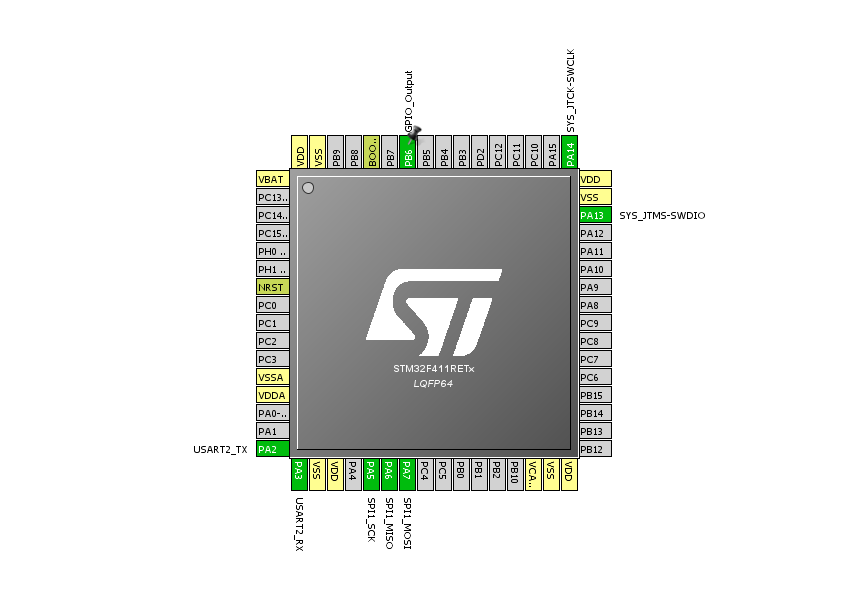
\includegraphics[width=400px]{img/cubemx.png}
    \caption{Praktinės dalies mikro-procesoriaus konfigūracija, naudojant STM32CubeMX \cite{STM3293:online}}
    \label{fig:stm32_cube_mx}
\end{figure}

Mikro-valdiklis sujungtas su jutikliu, naudojant SPI komunikacijos jungtį.
SPI jungtis reikalauja keturių jungčių -- laikrodžio (SCK), pasirinkimo (SS) ir dviejų duomenų linijų: MISO/MOSI.
MPU-9250 jutiklio specifikacijoje, šios kojos yra aprašomos kaip SCL, NCS, SDA ir AU0.
Iš paminėtų linijų, SCL jungiam prie SCK, NCS jungiam su SS, MISO jungiam su AU0 ir MOSI su SDA.
Tolimesnė SPI komunikacija yra vykdoma pagal protokolą.

Prieš pradedant bet kokių jutiklio duomenų nuskaitymą, būtina pasitikrinti ar komunikacija su jutikliu yra galima.
Tokiu tikslu jutikliui yra siunčiamas pasisveikinimo kodas -- \textit{0x75}.
Į kurį jutiklis turi atsakyti \textit{0x71}.
Jeigu atsakymas nėra toks -- vadinasi komunikacija nėra vykdoma ir jokie duomenų mainai nėra galimi.
Iš praktinės dalies galima paminėti, jog jeigu yra gaunamos kažkokios kraštutinės reikšmės -- \textit{0x00} arba \textit{0xFF}, SPI protokolo sujungimas visiškai nedirba ir problema tikrai bus arba litavime arba pačiuose kontaktuose, bet tikrai ne programinėje įrangoje.

Tolimesnis žingsnis yra normalizavimas.
Kiekvienas MPU-9250 yra normalizuojamas gamykloje, tačiau nėra pašalinama \textit{z} ašies gravitacinė komponentė.
Tai padaryta dėl to, kad skirtingose planetos vietose gravitacinė komponentė yra skirtinga, todėl jos normalizuoti nėra tikslo.
Kadangi vis tiek atliksime normalizavimą vienai ašiai -- galime iškarto normalizuoti ir likusias tris -- tiek linijinio, tiek kampinio pagreičio komponentes.

Normalizavimo proceso rezultatas yra nuolatinės dedamosios radimas.
Norint rasti nuolatinę dedamąja, reikia jutiklį paruošti -- jį korektiškai sukonfigūruoti, kad jis dirbtų prie savo galimų ribų.
Nustatyti žemo lygio filtrą iki $188 HZ$, pakelti mėginių rinkimo dažnį iki $1Khz$, kampinį pagreičio tikslumą nustatyti $250$ laipsnių per sekundę, o linijinį pagreičio tikslumą nustatyti $2g$.
Tuomet reikia surinkti pakankamą mėginių skaičių.
Skirtingi sprendimai renka skirtingus mėginių skaičių, todėl šiuo atveju bus pasirinkta $64$ mėginiai.
Tolimesnė eiga yra rasti visų mėginių vidurkį, pagal kiekvieną ašį.
Šitie skaičiai ir yra nuolatinės dedamosios komponentai. Juos reikia pašalinti iš gautų iš jutiklių duomenų.

Turint normalizuotus jutiklių duomenis, įmanomas duomenų rinkimas.
